\documentclass[../main.tex]{subfiles}
\begin{document}

\section{Partizioni}
Quindi per ogni partizione P, poniamo\[m_k = inf\{f(x):x\in [x_{k-1}, x_k]\}\]

\begin{figure}[ht]
    \centering
    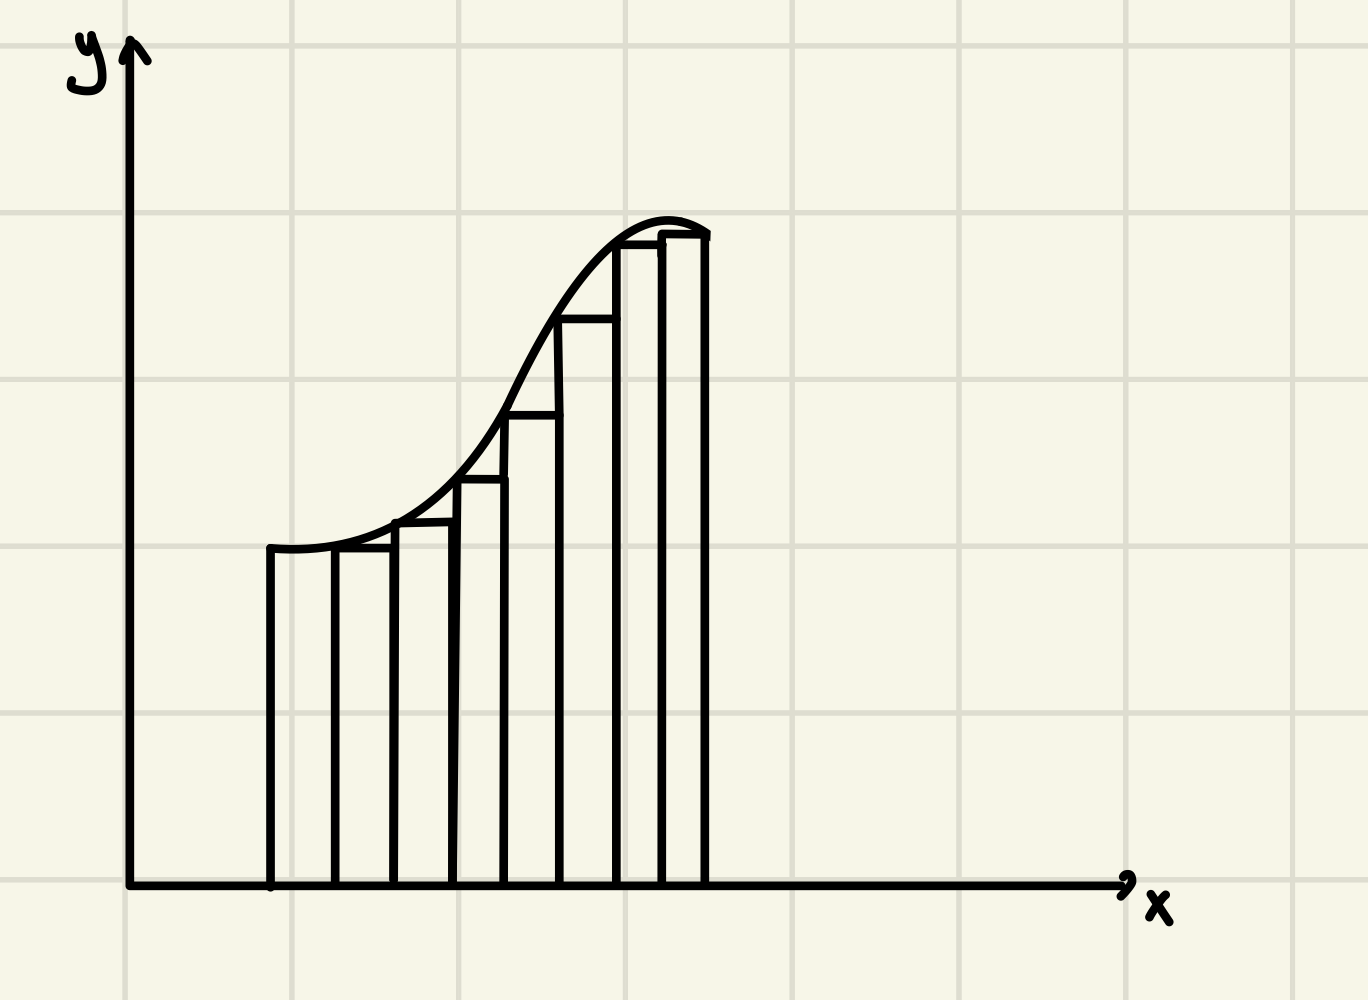
\includegraphics[width=0.3\linewidth]{inf.png}
    \caption{Inf}
    \label{fig:inf}
\end{figure}

(In questo caso è un minimo)

e poniamo\[M_k = sup\{f(x):x\in[x_{k-1}, x_k]\}\]

\begin{figure}[!ht]
    \centering
    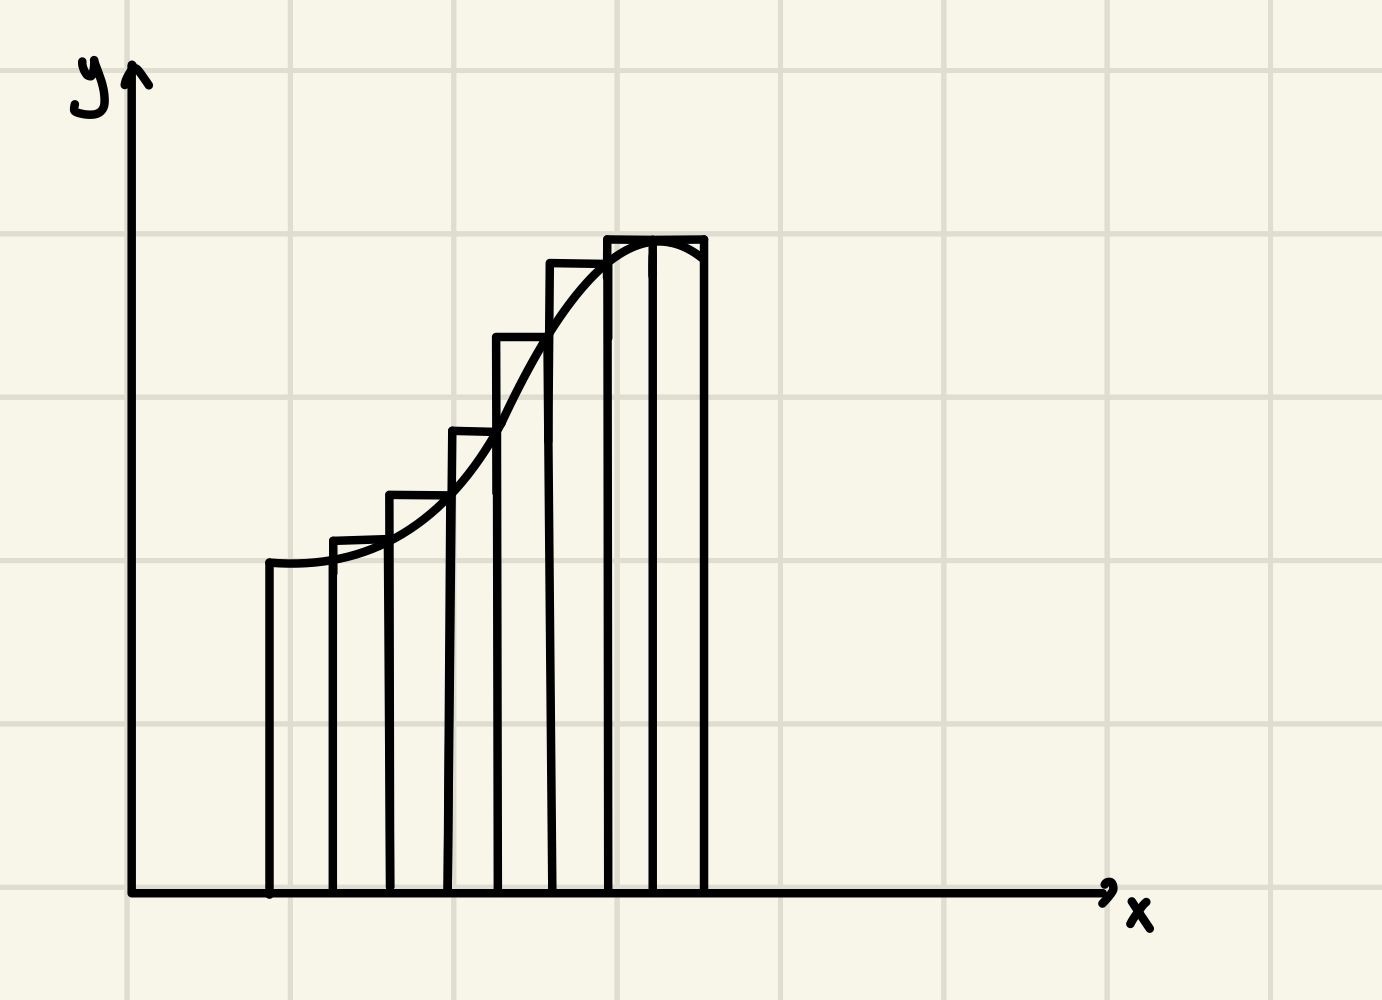
\includegraphics[width=0.3\linewidth]{sup.png}
    \caption{Sup}\label{fig:sup}
\end{figure}

(In questo caso è un massimo)

\newpage

Ad esempio:
\begin{figure}[ht]
    \centering
    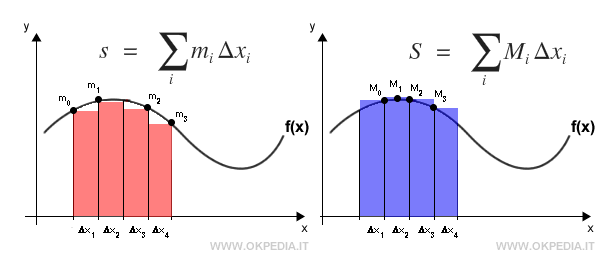
\includegraphics[width=0.5\linewidth]{image.png}\label{fig:supinf}
\end{figure}

\vspace{10pt}
In entrambe le figure sono rettangoli con la stessa base, ma con diversa
altezza. Sono aree per difetto e per eccesso della regione che voglio stimare.\\
Definisco le SOMME INTEGRALI INFERIORI: Somma delle aree dei rettangoli
inscritti.\[S(p) = \sum_{k=1}^{n}m_k(x_k-x_{k-1})\]
e le SOMME INTEGRALI SUPERIORI: Somma delle aree dei rettangoli circoscritti.
\[S(p) = \sum_{k=1}^{n}M_k(x_k-x_{k-1})\]

\subsection{Osservazione}
Se $f(x)$ è positiva, queste somme integrali sono la somma delle aree dei
rettangoli inscritti e circoscritti (sono definite a prescindere dal segno)

Si dimostra che:\[S(P) \leq S(P)\] e indicando con A l'insieme numerico descritto dalle somme integrali inferiori
$(P)$ al variare delle partizioni P dell'intervallo $[a, b]$ e con B l'insieme
delle corrispondenti somme superiori:\[A = \{s(P)\} \ \ \ B=\{S(P)\}\] si dimostra che A e B sono insiemi SEPARATI, cioè $A\leq B$:\[a\leq b \forall a\in A \ \ \land \ \ \forall b \in
    B\]

$\implies$ Dall'assioma di completezza segue che esiste almeno un numero reale c maggiore uguale a tutti gli elementi di A e minore o uguale a tutti gli elementi di B.
\[a\leq c \leq b\]
In generale questo elemento non è unico, e vale la seguente:

\section{Integrale definito}
Se l'elemento di separazione tra A e B è unico, allora si dice che f(x) è
INTEGRABILE SECONDO RIEMANN in $[a, b]$ e l'elemento si chiama con:\[\int_a^b
    f(x)dx\] e si chiama INTEGRALE DEFINITO di f in $[a, b]$. Quindi posto:\[S(f)
    = sup\{s(P) : P \ \ partizione \ \ di\ \ [a, b]\}\]\[S(f) = inf\{S(P) : P \ \
    partizione \ \ di\ \ [a, b]\}\] se $s(f) = S(P)$ $\rightarrow$ allora f(x) è integrabile secondo Riemann.

\subsection{Funzione non integrabile secondo Riemann}
Funzione di Dirichlet:
\begin{center}
    $f(x)$:
    $
        \begin{cases}
            0 & \qquad x\in \mathbb{Q}               \\
            1 & \qquad x \in \mathbb{R} - \mathbb{Q}
        \end{cases}
    $
\end{center}

\begin{figure}[!ht]
    \centering
    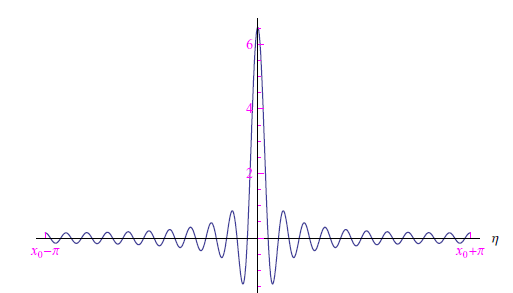
\includegraphics[width=0.5\linewidth]{dir.png}
    \caption{Funzione di Dirichlet}\label{fig:Dirichlet}
\end{figure}

In ogni intervallo $[x_{k-1}, x_k]$ cadono sia punti razionali che irrazionali:
\[m_k = inf\{f(x);x\in [x_{k-1}, x_k]\} = 0\]\[M_k = sup\{f(x);x\in [x_{k-1},
        x_k]\} = 1\] Allora: (somma integrali inferiori)\[S(P) = \sum_{k=1}^n
    0\cdot(x_k - x_{k-1}) = 0\]

\begin{align*}
    S(P) & = \sum_{k=1}^n 1\cdot(x_k - x_{k-1}) = (x_1-x_0)+(x_2-x_1)+(x_3-x_2) + \dotsb + (x_{n-1}-x_{n-2}) + (x_n - x_{n-1}) \\
         & = x_n - x_0 = b - a
\end{align*}
\vspace{2pt}

$\rightarrow S(P) = 0 \ \forall \ P \land S(P) = b-a \ \forall P$

Non è integrabile secondo Riemann.\ (lo sarà secondo LEBESGUE)

\newpage
\subsection{Proprietà}
\subsubsection{Additività integrale rispetto all'intervallo}
Se a,b,c sono tre punti di un intervallo dove la funzione f(x) è integrabile,
allora:\[\int_a^b f(x)dx = \int_a^c f(x)dx + \int_c^b f(x)dx\]

\begin{figure}[ht]
    \centering
    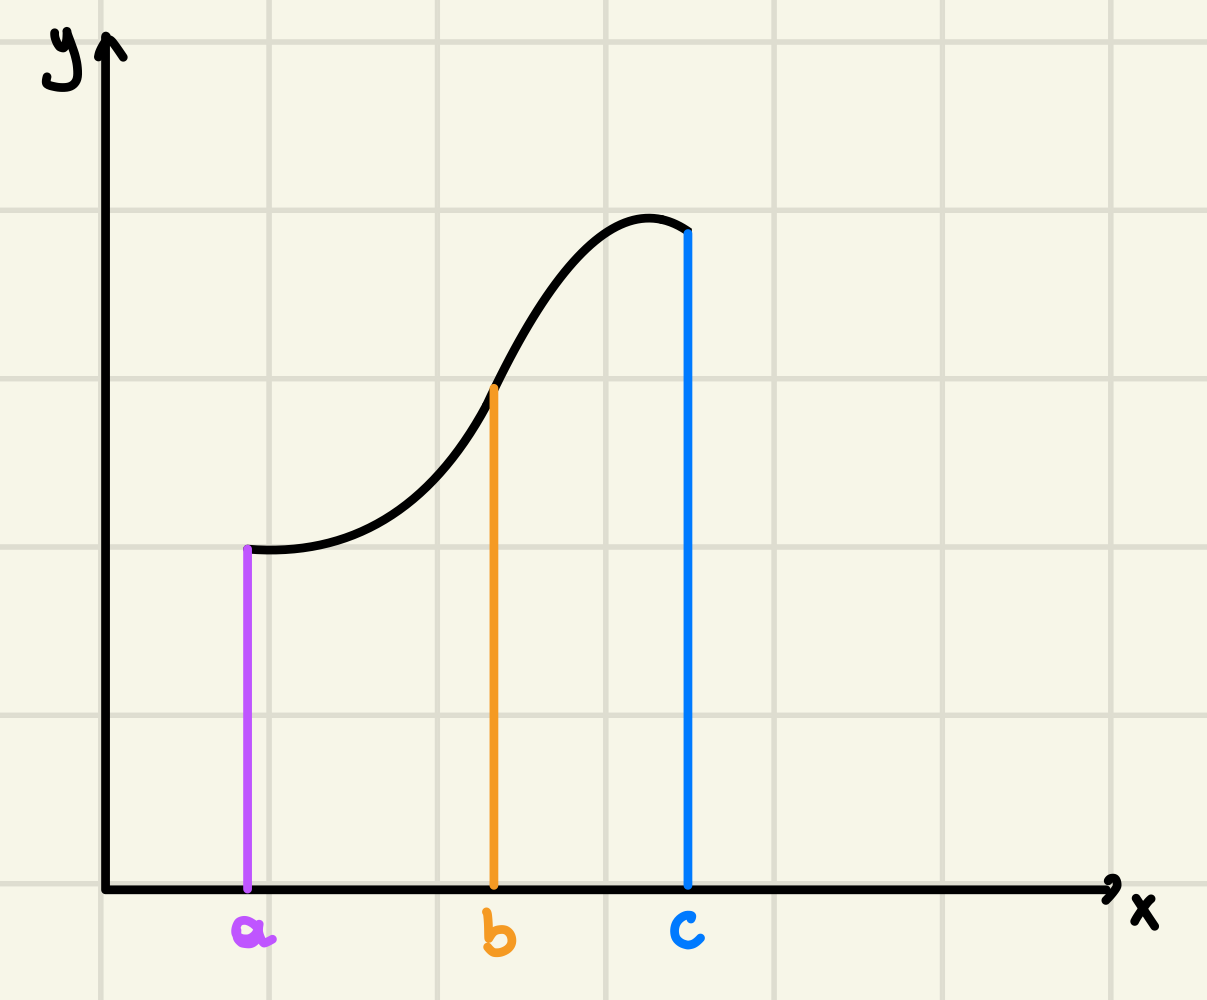
\includegraphics[width=0.3\linewidth]{abc.png}
    \caption{Grafico additività integrale}\label{fig:additivita-integrale}
\end{figure}

\subsubsection{Linearità dell'integrale}
Se f e g sono funzioni integrabili in $[a, b]$, anche $f+g$ è integrabile in
$[a, b]$. Dato c numero reale, anche $c\cdot f$ è integrabile in $[a, b]$.
\[\int_a^b [f(x)+g(x)]dx = \int_a^b f(x)dx + \int_a^b g(x)dx\]\[\int_a^b
    c\cdot f(x)dx = c\cdot\int_a^b f(x)dx\]

\subsubsection{Confronto tra gli integrali}
Se f e g sono funzioni integrabili in $[a, b]$ e se $f(x) \leq g(x) \forall x
    \in [a, b]$, allora:\[\int_a^b f(x)dx \leq \int_a^b g(x)dx\]

\subsubsection{Integrabilità delle funzioni continue}
Sia f(x) una funzione continua in $[a, b]$. Allora f(c) è integrabile secondo
Riemann in $[a, b]$.

\subsection{Teorema della media}
Se f(x) è continua in $[a, b]$, esiste un punto $x_0 \in [a, b]$ tale che:
\[\int_a^b f(x)dx = f(x_0)\cdot(b-a)\]

\newpage
\subsection{Interpretazione geometrica del teorema della media}
f(x) continua in $[a, b]$, ad esempio:

\begin{figure}[ht]
    \centering
    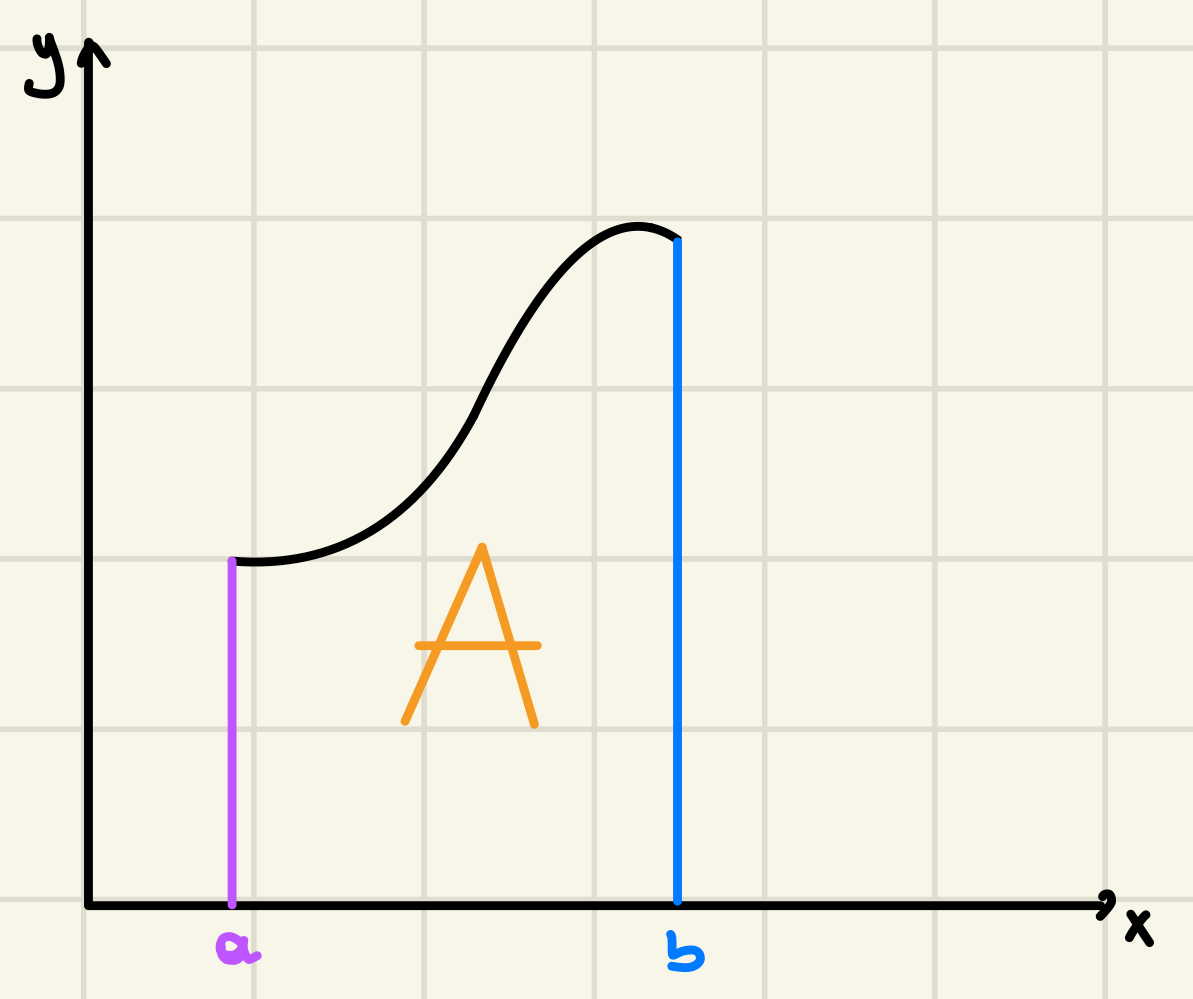
\includegraphics[width=0.5\linewidth]{fnz.png}\label{fig:teorema-media}
\end{figure}

Voglio calcolare l'area del rettangolo A. Il teorema della media afferma che
$\exists$ un valore opportuno (cioè un valore non scelto a caso, ma in base
alla particolare funzione considerata) f($x_0)$, tale che:

\begin{figure}[!ht]
    \centering
    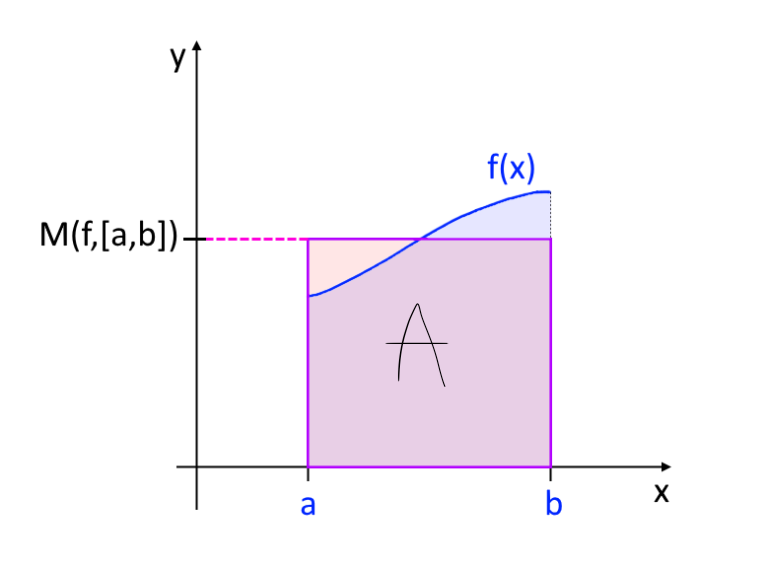
\includegraphics[width=0.5\linewidth]{media.png}
    \caption{Teorema della media}\label{fig:media}
\end{figure}

Per cui area A = area B, dove B è un rettangolo che ha per base l'intervallo
$[a, b]$ e per altezza $f(x_0)$.

\subsubsection{Dimostrazione del teorema della media}
f una funzione continua in $[a, b]$ per ipotesi. Per il teorema di Weierstrass
f(x) assume massimo e minimo in $[a, b]$, cioè esistono m e M tali che: (teo
esistenza valori intermedi)\[m\leq f(x) \leq M \forall x \in [a, b]\]

Consideriamo ora una partizione P di $[a, b]$, la più semplice possibile, cioè:
\[P = \{x_0 = a, x_1 = b\}\]

\begin{figure}[!ht]
    \centering
    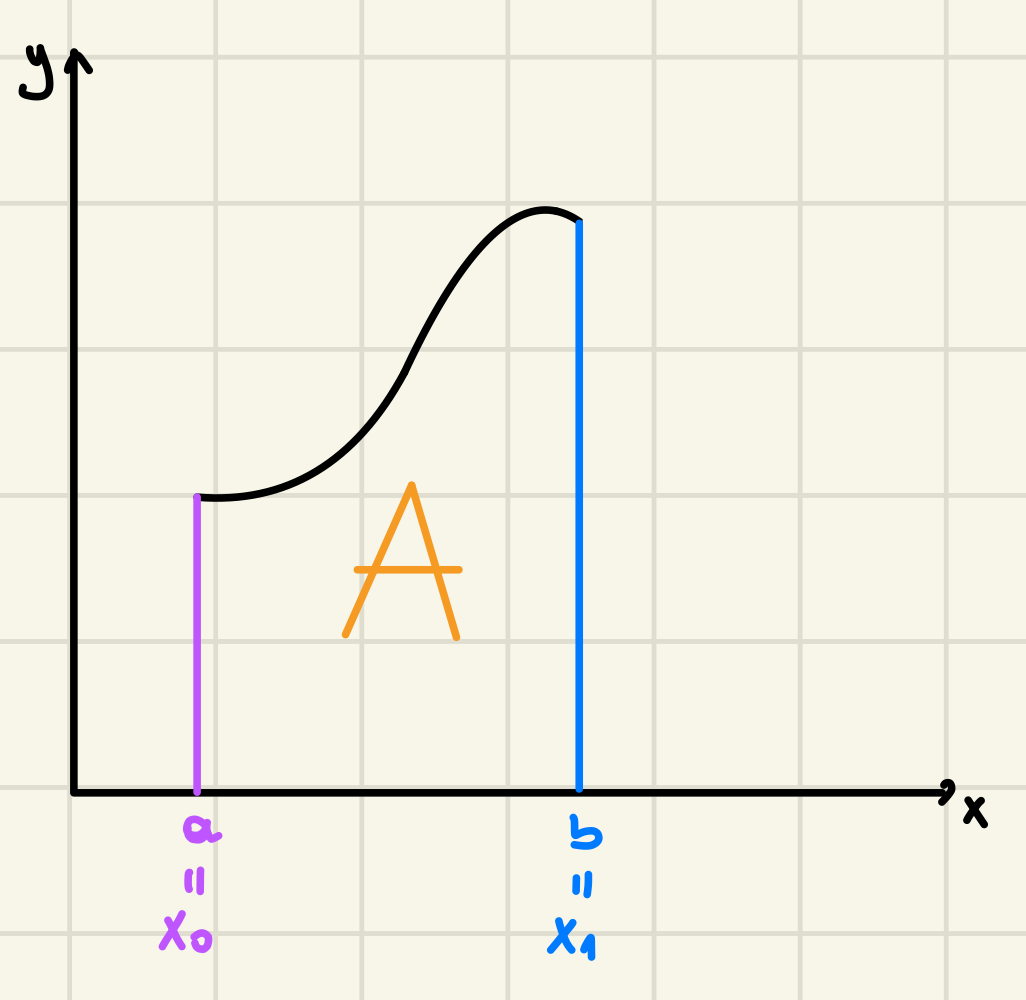
\includegraphics[width=0.3\linewidth]{x0x1.png}
    \caption{Enter Caption}\label{fig:enter-label}
\end{figure}

Le relative somme integrali inferiori e superiori sono date quindi da:\[s(P) =
    m(b-a)\]\[S(P) = M(b-a)\]

// grafico

L'integrale definito è, per definizione, l'elemento di separazione delle somme
integrali inferiori e delle somme integrali superiori (qualunque sia la
partizione P di $[a, b]$). Quindi:\[s(P) \leq \int_b^af(x)dx \leq S(P)\]
\[\rightarrow m(b-a) \leq \int_b^af(x)dx \leq M(b-a)\] se e solo se\[m \leq
    \frac{1}{b-a}\int_a^bf(x)dx \leq M\]\[\frac{1}{b-a}\int_a^bf(x)dx = y_0\]
$y_0$ è un numero compreso tra m ed M, minimo e massimo di f(x) $\implies$ per
il teorema di esistenza dei valori intermedi, $\exists x_0 \in [a, b] \ t.c.$
\[f(x_0)=y_0\]\[\implies f(x_0) = \frac{1}{b-a}\int_a^bf(x)dx\]
\[\frac{1}{b-a}\int_a^bf(x)dx = y_0\]

\[\implies \int_a^bf(x)dx = (b-a)f(x_0)\]

\subsection{Integrabilità delle funzioni monotone}
Sia f(x) una funzione monotona in $[a, b]$. Allora f(x) è integrabile secondo
Riemann in $[a, b]$ (indipendente dalle discontinuità) \\
\begin{figure}[ht]
    \centering
    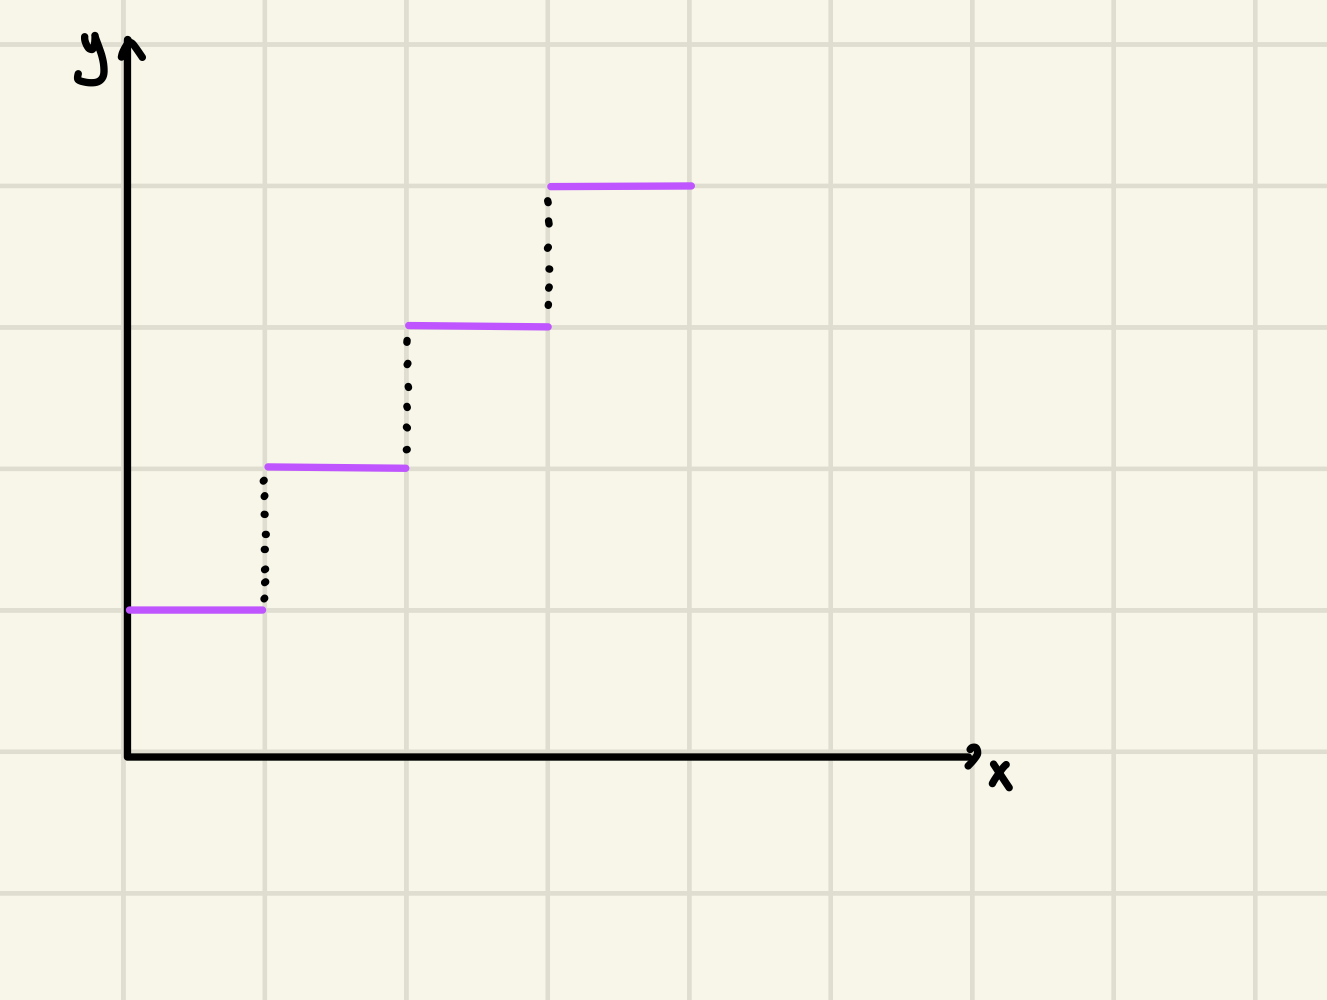
\includegraphics[width=0.3\linewidth]{scalini.png}
    \caption{funzione a scalini}
    \label{fig:enter-label}
\end{figure}

\subsubsection{Osservazioni}
In vista di andare a definire gli \textbf{INTEGRALI INDEFINITI}, concludiamo
con alcune notazioni e definizioni. Abbiamo definito l'integrale definito come:
\[\int_a^bf(x)dx\] dove a e b sono gli estremi di integrazione, la funzione f si dice funzione
\textbf{integranda}, la variabile x, si dice \textbf{variabile di
    integrazione}.

Notiamo che il risultato dell'integrazione non dipende da x, ma è un numero
reale. Poniamo inoltre per definizione:\[\int_a^bf(x)dx = - \int_b^af(x)dx \ \
    \ (a > b)\]
\begin{center}
    e
\end{center}

\[\int_a^af(x)dx = 0\]

\section{Integrali Indefiniti}
Mettiamo ora in evidenza, ma dei risultati più importati che lega le derivate
con gli integrali. Preliminarmente definiamo la FUNZIONE INTEGRALE.

\subsection{Funzione integrale}
Data f una funzione continua in $[a, b]$, definiamo:\[F(x) = \int_a^xf( )\]
qui $"x"$ è impegnato.

\[\implies F(x) = \int_a^xf(t)dt\]

\end{document}